\newpage
\subsection{UC10: Registrazione standard}
\label{sec:UC10}
\begin{figure}[!ht]
    \caption{Diagramma di UC10: Registrazione standard}
    \vspace{10px}
    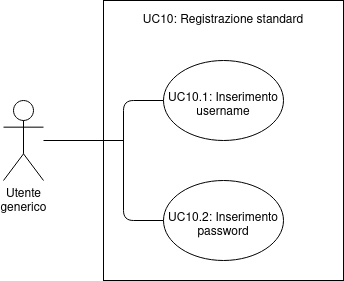
\includegraphics[scale=0.5]{../../../Images/AnalisiRequisiti/UC10}
    \centering
\end{figure}
\begin{itemize}
    \item \textbf{Descrizione:} l'utente vuole registrarsi nella piattaforma;
    \item \textbf{Attore Primario:} utente generico;
    \item \textbf{Attore Secondario:} servizio di autenticazione esterno;
    \item \textbf{Precondizione:} l'utente non ha un profilo nella piattaforma;
    \item \textbf{Input:} pressione apposito bottone;
    \item \textbf{Postcondizione:} l'utente ha effettuato la registrazione tramite servizio di autenticazione esterno. 
    \item \textbf{Scenario Principale:}
    \begin{itemize}
        \item un utente arriva per la prima volta nella piattaforma;
        \item si registra attraverso il servizio di autenticazione esterno, inserendo i seguenti dati:
        \begin{itemize}
            \item nome (\hyperref[sec:UC10.1]{\underline{UC10.1}});
            \item cognome (\hyperref[sec:UC10.2]{\underline{UC10.2}});
            \item username (\hyperref[sec:UC10.3]{\underline{UC10.3}});
            \item password (\hyperref[sec:UC10.4]{\underline{UC10.4}});
            \item ripetizione password.
        \end{itemize}
        \item l'utente è registrato.
    \end{itemize} 
\end{itemize}

\subsubsection{UC10.1: Inserimento nome}
\label{sec:UC10.1}
\begin{itemize}
    \item \textbf{Descrizione:} l'utente inserisce il nome per registrarsi;
    \item \textbf{Attore Primario:} utente generico;
    \item \textbf{Attore Secondario:} servizio di autenticazione esterno;
    \item \textbf{Precondizione:} l'utente ha iniziato la registrazione;
    \item \textbf{Input:} stringa con il nome;
    \item \textbf{Postcondizione:} l'utente ha inserito il nome. 
\end{itemize}

\subsubsection{UC10.2: Inserimento cognome}
\label{sec:UC10.2}
\begin{itemize}
    \item \textbf{Descrizione:} l'utente inserisce il cognome per registrarsi;
    \item \textbf{Attore Primario:} utente generico;
    \item \textbf{Attore Secondario:} servizio di autenticazione esterno;
    \item \textbf{Precondizione:} l'utente ha inserito il nome (\hyperref[sec:UC10.1]{\underline{UC10.1}});
    \item \textbf{Input:} stringa con il cognome;
    \item \textbf{Postcondizione:} l'utente ha inserito il cognome. 
\end{itemize}

\subsubsection{UC10.3: Inserimento username}
\label{sec:UC10.3}
\begin{itemize}
    \item \textbf{Descrizione:} l'utente inserisce lo username per registrarsi;
    \item \textbf{Attore Primario:} utente generico;
    \item \textbf{Attore Secondario:} servizio di autenticazione esterno;
    \item \textbf{Precondizione:} l'utente ha inserito il cognome (\hyperref[sec:UC10.2]{\underline{UC10.2}});
    \item \textbf{Input:} stringa con lo username;
    \item \textbf{Postcondizione:} l'utente ha inserito lo username.
    \item \textbf{Estensione:} 
    \begin{itemize}
        \item Se lo username è già utilizzato da un altro utente viene visualizzato un errore. (\hyperref[sec:UC10.5]{\underline{UC10.5}}) 
    \end{itemize} 
\end{itemize}

\subsubsection{UC10.4: Inserimento password}
\label{sec:UC10.4}
\begin{itemize}
    \item \textbf{Descrizione:} l'utente inserisce la password per registrarsi;
    \item \textbf{Attore Primario:} utente generico;
    \item \textbf{Attore Secondario:} servizio di autenticazione esterno;
    \item \textbf{Precondizione:} l'utente ha inserito lo username (\hyperref[sec:UC10.3]{\underline{UC10.3}});
    \item \textbf{Input:} stringa con la password;
    \item \textbf{Postcondizione:} l'utente ha inserito sia la password che la conferma.
    \item \textbf{Scenario Principale:}
        \begin{itemize}
            \item l'utente ha inserito tutti gli altri dati;
            \item l'utente inserisce la propria password;
            \item l'utente inserisce la conferma della password;
            \item l'utente termina la registrazione.
        \end{itemize} 
\end{itemize}

\subsubsection{UC10.5: Visualizzazione username già presente}
\label{sec:UC10.5}
\begin{itemize}
    \item \textbf{Descrizione:} Visualizzazione di un errore se lo username è già in uso;
    \item \textbf{Attore Primario:} utente generico;
    \item \textbf{Attore Secondario:} servizio di autenticazione esterno;
    \item \textbf{Precondizione:} l'utente ha inserito uno username non disponibile perchè già usato;
    \item \textbf{Postcondizione:} l'utente visualizza un messaggio di errore. 
\end{itemize}